\documentclass{article}
\usepackage[margin=0.18in,paperwidth=6.875in,paperheight=3.073in]{geometry}
\usepackage[T1]{fontenc}
\usepackage{lmodern}
\usepackage{tikz}
\usetikzlibrary{arrows.meta,positioning}
\pagestyle{empty}
\pagecolor{white}
\setlength{\parindent}{0pt}
\begin{document}
\centering
\vspace*{\fill}
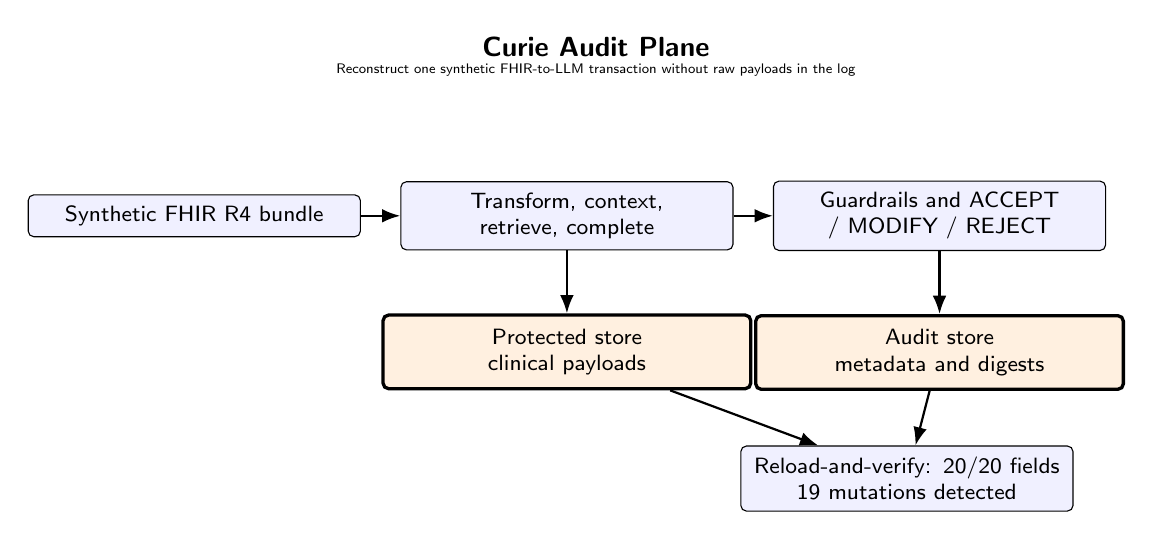
\begin{tikzpicture}[
  font=\sffamily\footnotesize,
  box/.style={draw, fill=blue!6, rounded corners=2pt, align=center, inner sep=4pt, text width=1.55in},
  store/.style={draw, very thick, fill=orange!12, rounded corners=2pt, align=center, inner sep=5pt, text width=1.7in},
  arr/.style={-{Latex}, thick}
]
\node[font=\sffamily\bfseries] at (5.1,2.15) {Curie Audit Plane};
\node[font=\sffamily\tiny] at (5.1,1.85) {Reconstruct one synthetic FHIR-to-LLM transaction without raw payloads in the log};
\node[box] (fhir) {Synthetic FHIR R4 bundle};
\node[box, right=5mm of fhir] (stages) {Transform, context, retrieve, complete};
\node[box, right=5mm of stages] (review) {Guardrails and ACCEPT / MODIFY / REJECT};
\draw[arr] (fhir) -- (stages);
\draw[arr] (stages) -- (review);
\node[store, below=8mm of stages] (prot) {Protected store\\clinical payloads};
\node[store, below=8mm of review] (audit) {Audit store\\metadata and digests};
\draw[arr] (stages) -- (prot);
\draw[arr] (review) -- (audit);
\node[box, below=7mm of prot, xshift=1.7in] (verify) {Reload-and-verify: 20/20 fields\\19 mutations detected};
\draw[arr] (prot) -- (verify);
\draw[arr] (audit) -- (verify);
\end{tikzpicture}
\vspace*{\fill}
\end{document}
